\documentclass[]{./tpl/isipfe}
\graphicspath{{./img/}}


\newenvironment{changemargin}[2]{%
\begin{list}{}{%
\setlength{\leftmargin}{#1}%
\setlength{\rightmargin}{#2}%
}%
\item[]}
{\end{list}}

\makeatletter

%================= front cover variables =================%

\newcommand{\secondAuthor}[1]{\gdef\@secondAuthor{#1}}%
\newcommand{\@secondAuthor}{\@latex@warning@no@line{No \noexpand\secondAuthor given}}

\newcommand{\diplomaName}[1]{\gdef\@diplomaName{#1}}%
\newcommand{\@diplomaName}{\@latex@warning@no@line{No \noexpand\diplomaName given}}

\newcommand{\speciality}[1]{\gdef\@speciality{#1}}%
\newcommand{\@speciality}{\@latex@warning@no@line{No \noexpand\speciality given}}

\newcommand{\proFramerName}[1]{\gdef\@proFramerName{#1}}%
\newcommand{\@proFramerName}{\@latex@warning@no@line{No \noexpand\proFramerName given}}

\newcommand{\proFramerSpeciality}[1]{\gdef\@proFramerSpeciality{#1}}%
\newcommand{\@proFramerSpeciality}{\@latex@warning@no@line{No \noexpand\proFramerSpeciality given}}

\newcommand{\academicFramerName}[1]{\gdef\@academicFramerName{#1}}%
\newcommand{\@academicFramerName}{\@latex@warning@no@line{No \noexpand\academicFramerName given}}

\newcommand{\academicFramerSpeciality}[1]{\gdef\@academicFramerSpeciality{#1}}%
\newcommand{\@academicFramerSpeciality}{\@latex@warning@no@line{No \noexpand\academicFramerSpeciality given}}

\newcommand{\collegeYear}[1]{\gdef\@collegeYear{#1}}%
\newcommand{\@collegeYear}{\@latex@warning@no@line{No \noexpand\collegeYear given}}

\newcommand{\companyName}[1]{\gdef\@companyName{#1}}%
\newcommand{\@companyName}{\@latex@warning@no@line{No \noexpand\companyName given}}

%================== Signatures variables ==================%

\newcommand{\proSignSentence}[1]{\gdef\@proSignSentence{#1}}%
\newcommand{\@proSignSentence}{\@latex@warning@no@line{No \noexpand\proSignSentence given}}

\newcommand{\academicSignSentence}[1]{\gdef\@academicSignSentence{#1}}%
\newcommand{\@academicSignSentence}{\@latex@warning@no@line{No \noexpand\academicSignSentence given}}

%================== Backcover variables ==================%

\newcommand{\arabicAbstract}[1]{\gdef\@arabicAbstract{#1}}%
\newcommand{\@arabicAbstract}{\@latex@warning@no@line{No \noexpand\arabicAbstract given}}

\newcommand{\arabicAbstractKeywords}[1]{\gdef\@arabicAbstractKeywords{#1}}%
\newcommand{\@arabicAbstractKeywords}{\@latex@warning@no@line{No \noexpand\arabicAbstractKeywords given}}

\newcommand{\frenchAbstract}[1]{\gdef\@frenchAbstract{#1}}%
\newcommand{\@frenchAbstract}{\@latex@warning@no@line{No \noexpand\frenchAbstract given}}

\newcommand{\frenchAbstractKeywords}[1]{\gdef\@frenchAbstractKeywords{#1}}%
\newcommand{\@frenchAbstractKeywords}{\@latex@warning@no@line{No \noexpand\frenchAbstractKeywords given}}

\newcommand{\englishAbstract}[1]{\gdef\@englishAbstract{#1}}%
\newcommand{\@englishAbstract}{\@latex@warning@no@line{No \noexpand\englishAbstract given}}

\newcommand{\englishAbstractKeywords}[1]{\gdef\@englishAbstractKeywords{#1}}%
\newcommand{\@englishAbstractKeywords}{\@latex@warning@no@line{No \noexpand\englishAbstractKeywords given}}

\newcommand{\companyEmail}[1]{\gdef\@companyEmail{#1}}%
\newcommand{\@companyEmail}{\@latex@warning@no@line{No \noexpand\companyEmail given}}

\newcommand{\companyTel}[1]{\gdef\@companyTel{#1}}%
\newcommand{\@companyTel}{\@latex@warning@no@line{No \noexpand\companyTel given}}

\newcommand{\companyFax}[1]{\gdef\@companyFax{#1}}%
\newcommand{\@companyFax}{\@latex@warning@no@line{No \noexpand\companyFax given}}

\newcommand{\companyAddressFR}[1]{\gdef\@companyAddressFR{#1}}%
\newcommand{\@companyAddressFR}{\@latex@warning@no@line{No \noexpand\companyAddressFR given}}

\newcommand{\companyAddressAR}[1]{\gdef\@companyAddressAR{#1}}%
\newcommand{\@companyAddressAR}{\@latex@warning@no@line{No \noexpand\companyAddressAR given}}

%============= cmd for inserting blank page =============%
\newcommand\blankpage{%
    \null
    \thispagestyle{empty}%
    \addtocounter{page}{-1}%
    \newpage}

%================ document main language ================%
%\selectlanguage{english}
\selectlanguage{french}

%================== required packages ===================%

\usepackage{tcolorbox}
\usepackage{afterpage}
\usepackage{array,longtable,multirow}% http://ctan.org/pkg/{array,longtable,multirow}
\usepackage{pifont}

\usepackage{pdflscape}
\usepackage{rotating}
\usepackage{wrapfig}
\usepackage{minitoc}

\usepackage{caption}
\usepackage{graphicx, threeparttable}
 \DeclareCaptionFormat{sanslabel}{#3}%


\makeindex
\usepackage{minitoc}
\begin{document}
\dominitoc
    %============= Config new columns type ==============%
\newcolumntype{L}{>{\raggedright\arraybackslash}}
\newcolumntype{R}{>{\raggedleft\arraybackslash}}
\newcolumntype{C}{>{\centering\arraybackslash}}
%==================================================%

%========= Config the cover section ==========%

\title{Titre du projet}

\author{Prénom NOM}


\diplomaName{Actuariat}
\speciality{Infini}

%% Encadrant professionnel
\proFramerName{Monsieur/Madame Prénom NOM}
\proFramerSpeciality{Ingénieur R\&D}

%% Encadrant académique
\academicFramerName{Monsieur/Madame Prénom NOM}
\academicFramerSpeciality{Maître Assistant(e)}

%% Entreprise d'accueil
\companyName{Tunisie Télécome}

%% Année universitaire
\collegeYear{2019 - 2020}

%%%%%% Signatures section %%%%%%

% You can simply remove theses sentences by typing an empty string
% \proSignSentence{}

\proSignSentence{J'autorise l'étudiant à faire le dépôt de son rapport de stage en vue d'une soutenance.}

\academicSignSentence{J'autorise l'étudiant à faire le dépôt de son rapport de stage en vue d'une soutenance.}

%%% AR
\arabicAbstract{يوضع الملخص باللغة العربية هنا... يوضع الملخص باللغة العربية هنا... يوضع الملخص باللغة العربية هنا... يوضع الملخص باللغة العربية هنا... يوضع الملخص باللغة العربية هنا... الرجاء أن يكون في حدود العشر أسطر... يوضع الملخص باللغة العربية هنا... الرجاء أن يكون في حدود العشر أسطر... يوضع الملخص باللغة العربية هنا... الرجاء أن يكون في حدود العشر أسطر... يوضع الملخص باللغة العربية هنا... الرجاء أن يكون في حدود العشر أسطر... يوضع الملخص باللغة العربية هنا... الرجاء أن يكون في حدود العشر أسطر... يوضع الملخص باللغة العربية هنا... الرجاء أن يكون في حدود العشر أسطر... يوضع الملخص باللغة العربية هنا... الرجاء أن يكون في حدود العشر أسطر... يمكنك أن تكتب كلمات بحروف لاتينية في وسط الملخص مثال \textLR{Exemple ici} يوضع الملخص باللغة العربية هنا...}

\arabicAbstractKeywords{الرجاء عدم تجاوز الخمس كلمات}

%% To use latin characters inside the arabic text
% just put them inside the command \textLR{}
%%%%

%%% FR
\frenchAbstract{Mettez le resumé en français ici... Mettez le resumé en français ici... Mettez le resumé en français ici... Mettez le resumé en français ici... Merci de ne pas dépasser les dix lignes. Mettez le resumé en français ici, merci de ne pas dépasser les dix lignes. Mettez le resumé en français ici, merci de ne pas dépasser les dix lignes. Mettez le resumé en français ici, merci de ne pas dépasser les dix lignes. Mettez le resumé en français ici, merci de ne pas dépasser les dix lignes. Mettez le resumé en français ici, merci de ne pas dépasser les dix lignes. Mettez le resumé en français ici, merci de ne pas dépasser les dix lignes. Mettez le resumé en français ici, merci de ne pas dépasser les dix lignes. Mettez le resumé en français ici, merci de ne pas dépasser les dix lignes.}

\frenchAbstractKeywords{Merci de ne pas dépasser les cinq mots}

%%% EN
\englishAbstract{Put the English abstract here, put the English abstract here, put the English abstract here, put the English abstract here, put the English abstract here, put the English abstract here... Please don't exceed ten lines, Please don't exceed ten lines, Please don't exceed ten lines, Please don't exceed ten lines. Put the English abstract here, please don't exceed ten lines. Put the English abstract here, please don't exceed ten lines. Put the English abstract here, please don't exceed ten lines. Put the English abstract here, please don't exceed ten lines. Put the English abstract here, please don't exceed ten lines. Put the English abstract here, please don't exceed ten lines. Put the English abstract here, please don't exceed ten lines. Put the English abstract here, please don't exceed ten lines.}

\englishAbstractKeywords{Please don't use more than five keywords}

%% if you want to get rid of the company address just set the boolean variable to false
% PS : it's optional
\setboolean{wantToTypeCompanyAddress}{true}

\companyEmail{contact@company.com}
\companyTel{71 111 111}
\companyFax{71 222 222}
\companyAddressAR{نهج بحيرة ملاران - ضفاف البحيرة - تونس}
\companyAddressFR{Rue du Lac Malaren, Les Berges du Lac 1053 Tunis}
    
    \frontmatter
        \thispagestyle{cover}%
\newgeometry{bottom=25mm,left=20mm,top=15mm,right=20mm}
\hspace{-47pt}
\begin{minipage}[l]{0.2\columnwidth}
\vspace{6mm}

\includegraphics[scale=0.4]{img/esprit.jpg}\\
\end{minipage}
\hfill
\begin{minipage}[l]{0.6\columnwidth}
\centering
\footnotesize
\hspace{2mm}
\textbf{{République Tunisienne}}\\
\vspace{1.5mm}
\textbf{{Ministère de l'Enseignement Supérieur\\
et de la Recherche Scientifique}}\\
\vspace{2mm}
\hspace{1cm}
\textbf{{Ecole Supérieure Privée d'Ingénierie et des Technologies}}\\
\vspace{1.5mm}

\end{minipage}
\hfill
\begin{minipage}[l]{0.02\columnwidth}
\end{minipage}
\hfill
\begin{minipage}[l]{0.2\columnwidth}
\vspace{6mm}

\end{minipage}
\vskip3cm

\begin{center}
{\LARGE{\textbf{\textsc{Rapport de Projet Actuariat Vie}}}}\\
\vskip0.5cm
\large

\end{center}

\begin{center}

   


\vskip15mm

\definecolor{isiBlue}{RGB}{31, 78, 121}

\begin{changemargin}{-9mm}{0cm}
\begin{minipage}[l]{1.1\columnwidth}
\begin{tcolorbox}[colframe=isiBlue,colback=white,boxrule=0pt,toprule=3pt,bottomrule=3pt,arc=0pt,top=0mm,right=0mm,left=0mm,bottom=0mm,boxsep=0.5mm]{
    \begin{tcolorbox}[colframe=isiBlue,colback=white, boxrule=0pt,toprule=1pt,bottomrule=1pt,arc=0pt,enlarge bottom by=-0.9mm, auto outer arc]
        \centering
        {\huge\textbf{Sujet 7 : Comparaison de deux modèles de mortalité}}
    \end{tcolorbox}
}
\end{tcolorbox}
\end{minipage}
\end{changemargin}
\vskip30mm
\textrm{Réalisé par}\\
\vskip0.3cm

        \begin{center}
            \large\textbf{Adam KAAK }\\
            \large\textbf{Amira CHEHAIBI}\\
            \large\textbf{Hechem BEN FARHAT}\\
            \large\textbf{Mohamed JAOUA}\\
            \large\textbf{Mohamed Yahia BOURGUIBA}
        \end{center}
    
\end{center}
\vskip8mm%



\vskip16mm



\afterpage{\blankpage}
       
        
        
       
        \thispagestyle{frontmatter}
        
       \setcounter{secnumdepth}{3}
        \setcounter{tocdepth}{2}
        \dominitoc
        \tableofcontents
        \adjustmtc
        \thispagestyle{frontmatter}
        
        \listoffigures
        \thispagestyle{frontmatter}
       % \listoftables
        \thispagestyle{frontmatter}
        
        \chapter*{Liste des abréviations}

\begin{acronyms}
    
    \sortitem[LCA]{
        \textbf{L}ee-\textbf{C}\textbf{A}rter
    }
    
    \sortitem[CBD]{
       \textbf{C}airns \textbf{B}lake \textbf{D}owd
    }
    
    \sortitem[OMS]{
     \textbf{O}rganisation \textbf{M}ondiale  de la\textbf{S}anté
    }
    
     \sortitem[HMD]{
      \textbf{H}uman \textbf{M}ortality \textbf{D}atabase 
    }
     \sortitem[ESPRIT]{
      \textbf{E}cole \textbf{S}upérieure \textbf{P}rivée d'\textbf{I}ngénierie et de \textbf{T}echnologie
    }
    
\end{acronyms}
        \thispagestyle{frontmatter}
    
    \mainmatter
        \chapter*{Introduction générale}
\par La population danoise représente environ 5 750 000 habitants, ce qui équivaut à 1,1$\%$ de la
population européenne. Avec 5 447 000 habitants en 2007 et 5 560000 en 2011, elle a un taux de croissance de 0,7$\%$ et augmente plus rapidement que dans le reste de l’Union européenne. Comme dans l’ensemble de la région nordique, à un vieillissement de la population plus élevé que dans les autres pays de l’Union s’ajoute une ouverture importante à l’immigration.

\par Avec 19,43$\%$ de la population ayant 65 ans ou plus, le Danemark est le onzième pays avec la population la plus âgée dans le monde. La part des 65-79 ans est celle qui a le plus augmenté depuis dix ans, passant de 11.1$\%$ de la population en 2006 à 14.6$\%$. Les projections prévoient une augmentation importante de la classe la plus âgée : la part des plus de 70 ans augmenterait de 64$\%$ entre 2017 et 2050.

\par L’espérance de vie des Danoises à la naissance est la plus faible parmi les treize pays européens pour lesquels on dispose de données en 1999 (c’est-à-dire sans l’Italie et la Grèce) et les résultats en termes d’espérance de vie masculine sont relativement peu satisfaisants. On retrouve le même phénomène lorsqu’on analyse l’espérance de vie à 65 ans, à la fois pour les hommes et pour les femmes.

\par Le Danemark se singularise ainsi des autres pays européens dans la mesure où, entre 1980 et 1995, l’espérance de vie à la naissance des femmes n’a progressé que de 6 mois.
Le taux de mortalité infantile et son evolution depuis 1980 confirment ces résultats sanitaires plutôt décevants ; en
effet, alors que le taux de mortalité infantile était relativement faible au Danemark en
1980, les progrès réalisés y ont été beaucoup plus lents que dans les autres pays européens 

\par D’autres éléments, liés aux comportements et aux modes de vie, sont également intéressants à noter. Le taux de mortalité par cancer est, par exemple, largement supérieur à celui observé dans les autres
pays (222 décès sur 100 000, contre 159 en Finlande et en Suède), mais l’incidencedes cancers y est aussi supérieure (561 cas pour 100 000, contre 420 en Finlande et 483 en Suède). 
Une étude parue dans le British Medical Journal en 20003 met en évidence la forte mortalité associée au tabac chez les femmes. Si, durant les années cinquante, le tabac était responsable de
1 $\%$ des décès des femmes entre 55 et 84 ans, en 1990 ce chiffre s’élevait à un quart des décès.
Les chiffres publiés par l’OMS(Organisation mondiale de la santé) sur les causes de décès corroborent cette analyse.
Le Danemark arrive en tête des pays européens en ce qui concerne les décès liés à l’alcool pour les femmes et deuxième pour les décès liés au tabac.
        \clearpage
        \dominitoc
        \setcounter{minitocdepth}{9}
        \chapter{Contexte général du projet}

\section*{Introduction}
Ce chapitre est consacré à la présentation générale du projet. Nous commençons par l'explication des motivations pour entreprendre ce projet. Ensuite, nous focalisons sur les objectifs de notre sujet et la solution proposée après avoir discuté la problématique à résoudre.
\section{Motivation}
Les Danois vivent plus longtemps que jamais. En 2016, l’espérance de vie à la naissance des Danois a atteint 78,8 ans pour les hommes et 82,8 ans pour les femmes. Depuis 2000, les hommes ont ainsi gagné 4,5 ans d’espérance de vie et les femmes 3,8 ans, grâce notamment à la baisse de la mortalité. Les gains obtenus par les femmes sont moins rapides que ceux des hommes et l’écart entre les sexes se resserre : de 4 ans et 7 mois en 2000, il est passé à 4 ans en 2016.

L’espérance de vie à 67 ans progresse également. Selon les dernières estimations de l’agence nationale Danmarks Statistik, les hommes danois âgés de 67 peuvent espérer de vivre encore 16,6 ans et les femmes 19,1 ans. Cela constitue depuis 2000 un gain de 2,9 ans pour les hommes et de 2,4 ans pour les femmes, donc à nouveau un rétrécissement de l’écart entre les sexes.

C'est pour cela que nous nous intéressons à ce sujet afin d'estimer et de projeter la mortalité de la population danoise (hommes et femmes) pour des âges supérieurs à 50 ans.

\section{Planification du projet}
\subsection{Objectif général}
L’objectif du projet est d'estimer et de prédire le taux de mortalité d'un groupe de danois avec 2 modèles différents: 
\begin{itemize}
    \item[*] Le modèle de Lee-Carter.
    \item[*] Le modèle de Cairns Blake Dowd (CBD).
\end{itemize}
\subsection{Planification prévisionnelle du projet}
Pour assurer le bon déroulement et l'avancement du travail on a mis en place une planification qui s'étale en 3 étapes selon les besoins spécifiques décrits précédemment.
\begin{itemize}
\item[*] \textit{Du 6-9 Mai } Exploitation et compréhension des données. 
    \item[*] \textit{Du 10-16 Mai} Compréhension des notations et préliminaires actuariels.
    \item[*] \textit{Du 17-30 Mai } Codage sous R et Rédaction du rapport en parallèle.
    
\end{itemize}
\section*{Conclusion}
Dans ce qui précède, nous avons abordées le contexte général de ce projet et plus
précisément l’environnement de réalisation. De même, nous avons précisées les objectifs du projet par une planification prévisionnelle qui nous a permis d’assurer le bon déroulement du travail et de garantir le respect des délais.


        %\clearpage
        
        \chapter{Vue d'ensemble des notions actuarielles}
\section*{Introduction}
Dans ce chapitre, On va introduire le modèle de Lee-Carter, le modèle de Cairns Blake Dowd (CBD) et la notion de taux de mortalité.
\section{Taux de mortalité}
\par Un taux de mortalité est une mesure de la fréquence des décès dans une population définie au cours d'un intervalle spécifié. Les mesures de morbidité et de mortalité sont souvent les mêmes mathématiquement; c'est juste une question de ce que vous choisissez de mesurer, la maladie ou la mort. 
\par Le taux de mortalité à l’âge x d’un individu est notée $\mu_x$, La formule de mortalité d'une population définie, sur une période de temps spécifiée, est donnée par \cite{cours} :
\begin{equation}
    \mu_{x+t} = \frac{f_x}{S_x}
\end{equation}
  Avec , 
    
    \begin{itemize}
        \item la fonction de répartition $F_x(t) = P(T_x < t | T_x > 0) = tq_x$,
        \item la fonction de survie $S_x(t) = P(Tx > t | T_x > 0) = tp_x$.
    \end{itemize}

\section{Modèle de Lee-Carter}
Il s’agit d’une méthode d’extrapolation des tendances passées initialement utilisée
sur des données américaines, qui est devenue rapidement un standard. La
modélisation retenue pour le taux instantané de mortalité est la suivante : 
\begin{equation}
\ln \mu_{xt} = \alpha_x + \beta_x\kappa_t + \epsilon_{xt}
\end{equation}
où :

- \textbf{$\mu_{xt}$} représente le taux instantané de mortalité à la date t pour l’âge x.

- \textbf{$\alpha_x$} est la composante spécifique à l’âge x, elle s’interprète comme la valeur
moyenne des \textbf{$\ln \mu_{xt}$} au cours du temps.

- \textbf{$\kappa_t$} décrit l’évolution générale de la mortalité.

- \textbf{$\beta_x$} traduit la sensibilité de la mortalité instantanée à l’âge x par rapport à l’évolution générale \textbf{$\kappa_t$} au sens où \begin{equation}\frac{\partial \ln(\mu_{xt})}{\partial \kappa_t} = \beta_x
\end{equation}

Ainsi, les âges pour lesquels les \textbf{$\beta_x$} sont importants sont les plus sensibles à l’évolution générale de la mortalité. Le modèle de Lee-Carter suppose la constance au cours du temps de cette sensibilité.

- \textbf{$\epsilon_{xt}$} est une variable aléatoire iid distribuée selon une loi $\mathcal{N}(0,\,\sigma^{2})$. 

L’idée du modèle est donc d’ajuster à la série (doublement indicée par x et t) des logarithmes des taux instantanés de décès une structure paramétrique(déterministe) à laquelle s’ajoute un phénomène aléatoire ; le critère d’optimisation retenu va consister à maximiser la variance expliquée par le modèle, ce qui revient à minimiser la variance des erreurs.
Afin de rendre le modèle identifiable, il convient d’ajouter des contraintes sur les paramètres ; on retient en général les contraintes suivantes :
\begin{equation}
\sum_{x=x_m}^{x_M} \beta_x = 1
\end{equation}
\begin{equation}
\sum_{t=t_m}^{t_M} \kappa_t = 0
\end{equation}

avec $t_m$ désignant la première année d’observation des taux de mortalité et $t_M$ la
dernière année de l’étude.
On obtient alors les paramètres par un critère de moindres carrés :  \begin{equation}
(\hat{\alpha_x},\hat{\beta_x},\hat{\kappa_x}) = arg min \sum_{x,t} (\ln \hat{\mu_{xt}}-\alpha_x - \beta_x \kappa_t)^2
\end{equation}

Il convient alors de résoudre ce programme d’optimisation, sous les contraintes d’identifiabilité. Le nombre de paramètres à estimer est élevé, il est égal à
\begin{equation} 
2(x_M - x-m + 1) + t_M - t_m -1
\end{equation}

\section{Procédure d'estimation du modèle Lee-Carter}
\subsection{Etape 1: Estimation des paramètres partir des données historiques}
Le modèle n'est pas un modèle de régression classique car ni $(\kappa_t)$ ni $(\beta_x)$  ne sont des paramètres observables.
Le but est l'estimation par méthode des moindres carrés en minimisant:
\begin{equation}
  \min_{\alpha_x,\beta_x,\kappa_t} \sum_{t=1}^{n} \sum_{x=x_min}^{x_max}(\log(\mu_x,t)-\alpha_x-\beta_x\kappa_t)^2
\end{equation}

La procédure est la décomposition en valeur singulière (SVD):
\begin{equation}
\hat{\alpha_x} = \frac{1}{n} \sum_{t=1}^{n} \log(\mu_{x,t})
\end{equation}

\subsection{Etape 2: Projection de la force de mortalité future}
\begin{equation}
log(\mu(x,t)) = \alpha_x + \beta_x\kappa_t
\end{equation}
Pour projeter la mortalité, il suffit de projeter la série temporelle $(\kappa_t)$
Les valeurs de $(\kappa_t)$ peuvent être modélisées par une série chronologique.
Exemple populaire: marche aléatoire avec tendance
\begin{equation}
\kappa_t = d + \kappa_{t-1} + \epsilon_t
\end{equation}
On peut obtenir des intervalles de confiance en simulant les
trajectoires de $(\kappa_t)$.
\section{Modèle de Cairns Blake Dowd (CBD)}
Nous avons considéré la formulation originale du modèle fourni par Cairns et al.(2006) avec le
équation de modèle suivante:
\begin{equation}
\ln[\frac{q_{x,t}}{p_{x,t}}] = k_t^{(1)} + k_t^{(2)} (x - \bar{x}) + \epsilon_{x,t}
\end{equation}
où
$k_t^{(1)}$ et $k_t^{(2)}$ sont deux processus stochastiques et représentent les deux indices temporels du modèle;
$q_{x,t}$ et $p_{x,t}$ représentent respectivement le décès et la probabilité de survie, au temps t pour un individu âgé de x;

\begin{equation}
\ln[\frac{q_{x,t}}{p_{x,t}}] = \ln(\phi_x) = logit q_{x,t}
\end{equation} est la transformation logit de $q_{x,t}$
, avec $\phi_x$ représentant les probabilités de mortalité;
$\bar{x}$ est l'âge moyen de l'intervalle d'âge considéré; et
$\epsilon_{x,t}$ est le terme d'erreur qui englobe la tendance historique que le modèle n'exprime pas. La totalité des termes d'erreur sont i.i.d suivant la distribution normale avec moyenne 0 et variance $\sigma^2$.

Le modèle est entièrement identifié, il ne nécessite donc pas de contraintes supplémentaires.
De plus, l'indice de temps $k_t^{(1)}$ est l'interception du modèle. Il affecte tous les âges de la même manière, et il représente le niveau de mortalité au temps t. Plus précisément, s'il diminue avec le temps, cela signifie que le taux de mortalité a diminué avec le temps à tous les âges. L'indice de temps $k_t^{(2)}$ représente la pente du modèle: chaque âge est affecté différemment par ce paramètre. Par exemple, si pendant la période d'essayage,
les améliorations de la mortalité ont été plus importantes à des âges inférieurs qu'à des âges plus élevés, le terme de période de pente
$k_t^{(2)}$ augmenterait avec le temps. Dans un tel cas, le graphique du logit des probabilités de décès par rapport à l'âge deviendrait plus raide à mesure qu'il se déplaçait vers le bas avec le temps (Pitacco et al.2009)


\section*{Conclusion}
Au cours de la section précédente, nous avons défini les différentes notions de l'actuariat vie que nous allons utiliser dans ce qui suit.
        \clearpage
        
        \chapter{Vue d'ensemble des notions actuarielles}
\section*{Introduction}
Dans ce chapitre on va parler de la réalisation des estimations ainsi que nos analyses et remarques.
\section{Lecture de données}
Comme indiqué dans l’énoncé on va travailler sur la population danoise bien évidemment notre pays concerné c’est le Danemark. Pour ce faire nous avons eu recours au site Human Mortality Database (HMD). C’est une base de données qui a été créée pour fournir des données détaillées sur la mortalité et la population aux chercheurs, étudiants, journalistes,
analystes des politiques et autres personnes intéressées par l’histoire de la longévité humaine.
on a utilisé la commande hmd.mx()pour le téléchargement. 

\section{Estimation des paramètres d’un modèle de Lee-Carter à partir des données historiques téléchargées}

\begin{figure}[!htb]
 \caption{Taux de mortalité des hommes danois entre 1876 et 2019}
    \centering
    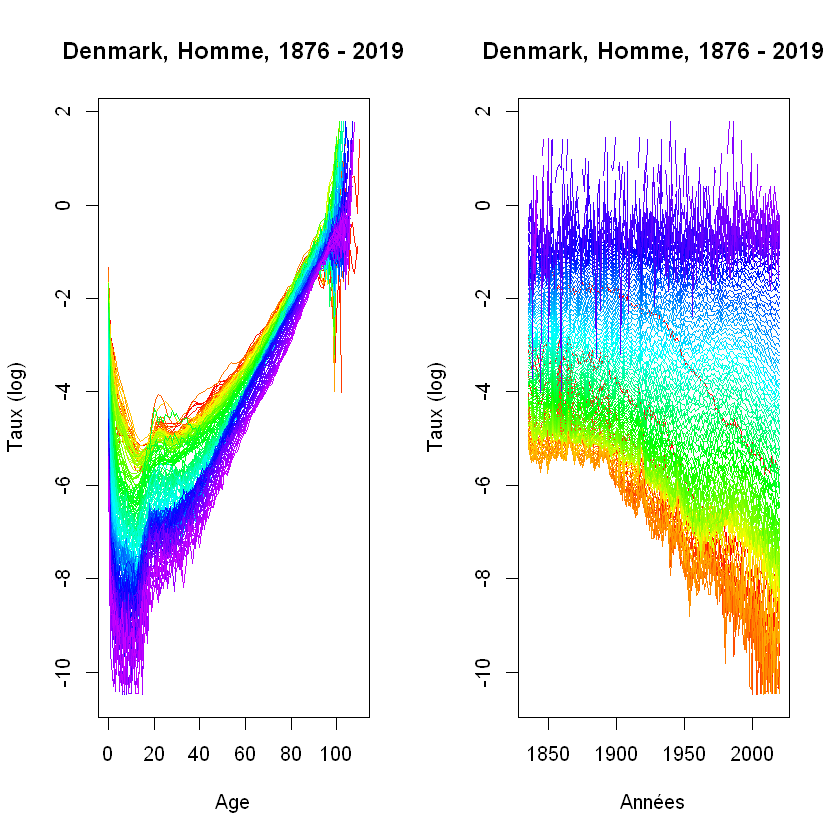
\includegraphics[scale =0.7]{output_7_0.png}
\end{figure}

\begin{figure}[!htb]
 \caption{Taux de mortalité des femmes danois entre 1876 et 2019}
    \centering
    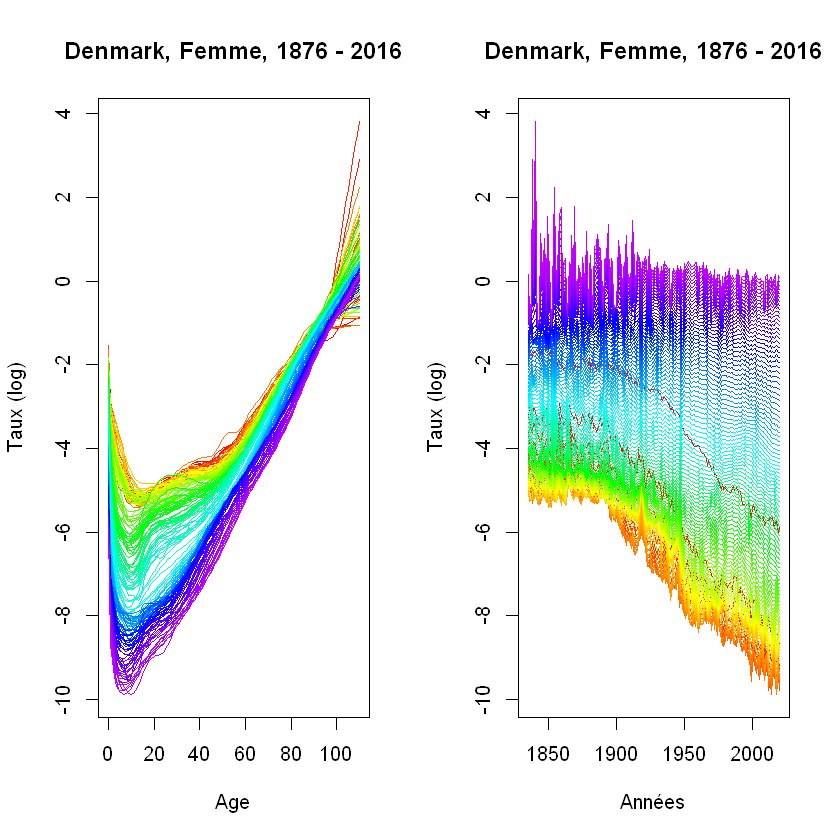
\includegraphics[scale =0.65]{output_7_1.png}
\end{figure}

\begin{figure}[!htb]
 \caption{Danemark, Effets principaux et interactions, Homme 1876-2019}
    \centering
    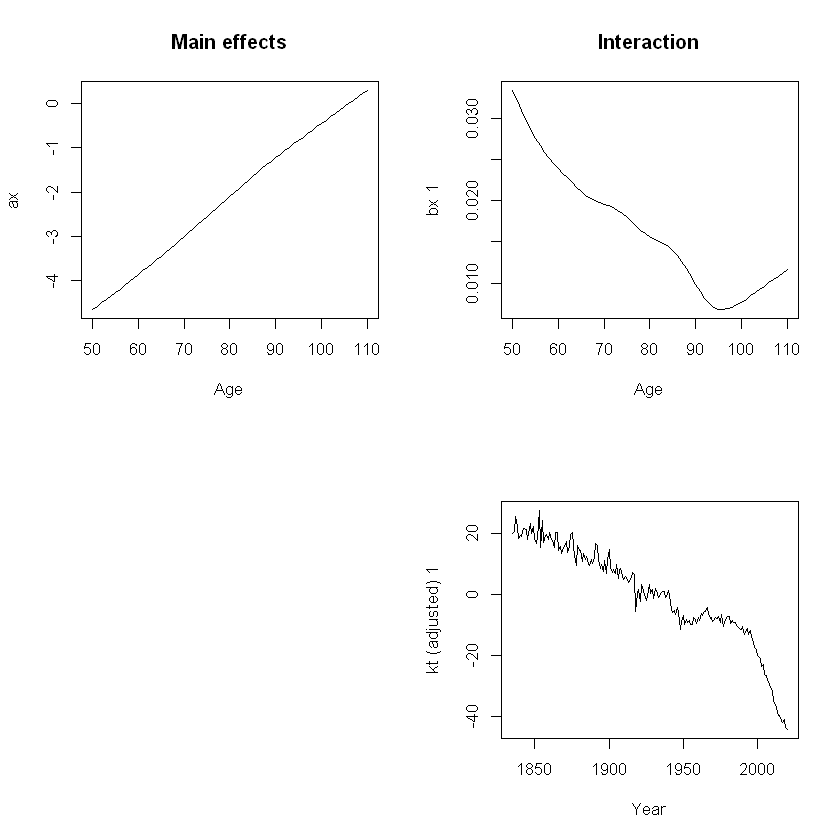
\includegraphics[scale =0.65]{output_7_3.png}
\end{figure}

\begin{figure}[!htb]
 \caption{Danemark, Effets principaux et interactions, Femme 1876-2019}
    \centering
    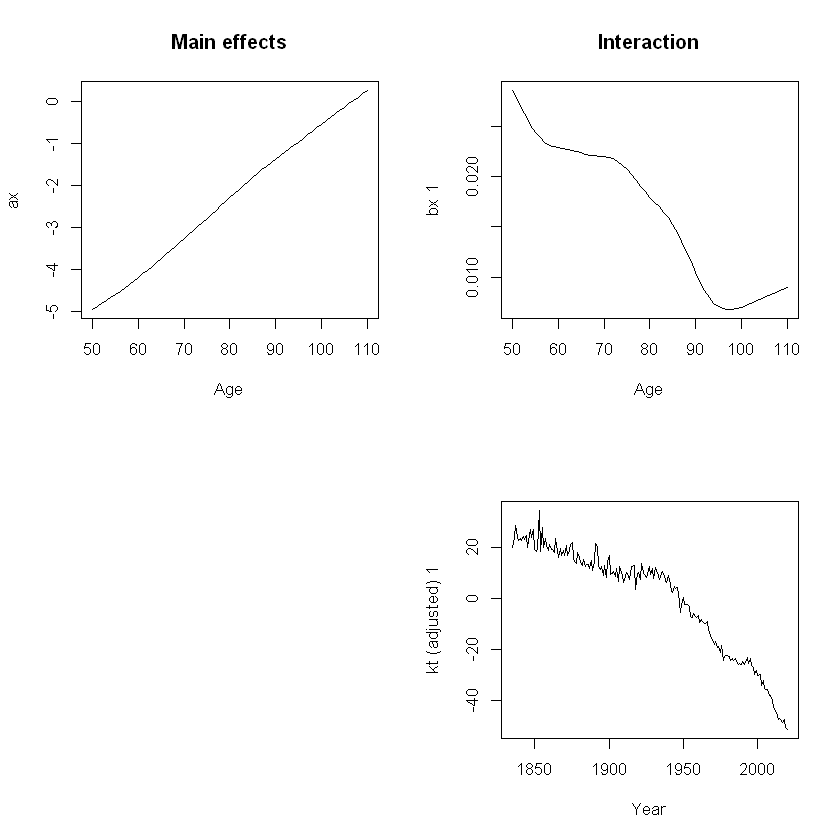
\includegraphics[scale =0.8]{output_7_5.png}
\end{figure}

Analyse des paramètres Pour Femme : ax : la valeur moyenne des logs de la mortalité instantanné ( ln µ(x,t) au cours du temps ) elle crois en fonction de l’age elle varie entre -5 et 0 .

bx indique la sensibilité de la mortalité instantanée par rapport à l’évolution générale de la mortalité. Si on se situe à partir de 55 ans, on constate que les âges les plus sensibles à l’évolution temporelle de la mortalité sont ceux entre 55 et 70 ans . On atteint en effet des stabilités sur ces tranches d’âges.

D’après la figure ci-dessus et comme kt indique l’évolution générale de la mortalité dans le temps ; On constate pendant les années 1860 une forte croissance due à la Seconde guerre du Schleswig qui c'est déroulé pendant la même periode . On constate une tendance linéaire à la décroissance des entre 1940 et 2010 Cette tendance à la décroissance du paramètre k, qui devient négatif au cours de la période, associée à la positivité moyenne du paramètre $\beta$ implique d’après la formule de Lee-Carter, une diminution des taux instantanés de mortalité. En conséquence, on assiste à une augmentation de la probabilité de la survie sur la période observée.

Analyse des paramètres Pour Homme : ax : la valeur moyenne des logs de la mortalité instantanné ( ln µ(x,t) au cours du temps ) elle crois en fonction de l’age elle varie entre -4 et 0 .

bx indique la sensibilité de la mortalité instantanée par rapport à l’évolution générale de la mortalité. on se situe à partir de 55 ans .

D’après la figure ci-dessus et comme kt indique l’évolution générale de la mortalité dans le temps ; On constate pendant les années 1860 une forte croissance due à la Seconde guerre du Schleswig qui c'est déroulé pendant la même periode . On constate une tendance linéaire à la décroissance des entre 1940 et 2010 Cette tendance à la décroissance du paramètre k, qui devient négatif au cours de la période, associée à la positivité moyenne du paramètre $\beta$ implique d’après la formule de Lee-Carter, une diminution des taux instantanés de mortalité. En conséquence, on assiste à une augmentation de la probabilité de la survie sur la période observée.

\begin{figure}[!htb]
 \caption{Le résidus du modèle LCA Pour Homme}
    \centering
    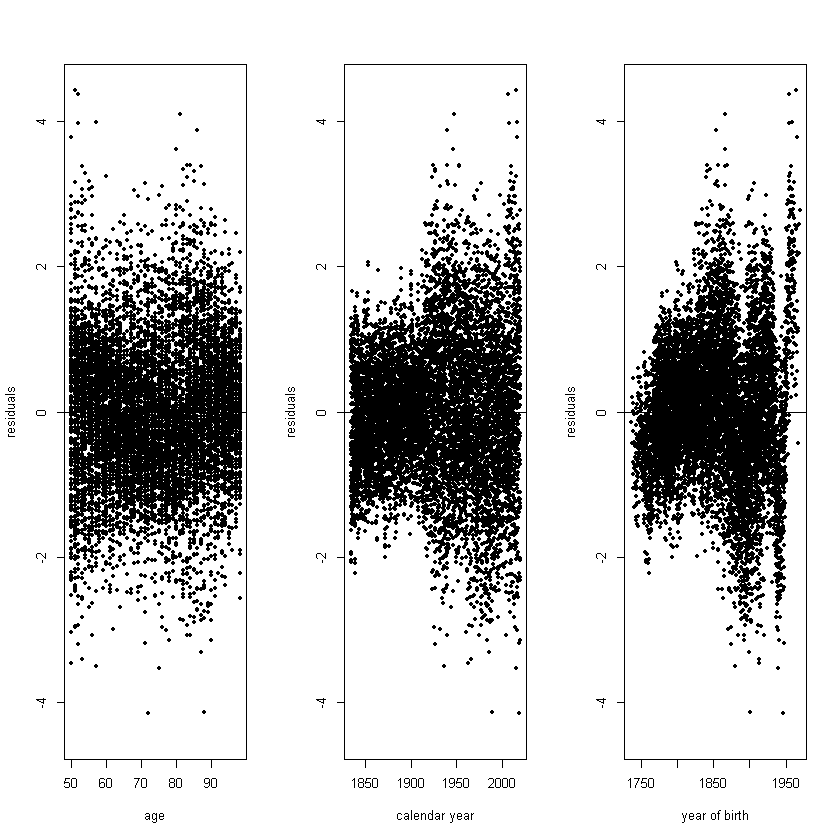
\includegraphics[scale =0.9]{output_9_1.png}
\end{figure}

\begin{figure}[!htb]
 \caption{Le résidus du modèle LCA Pour Femme}
    \centering
    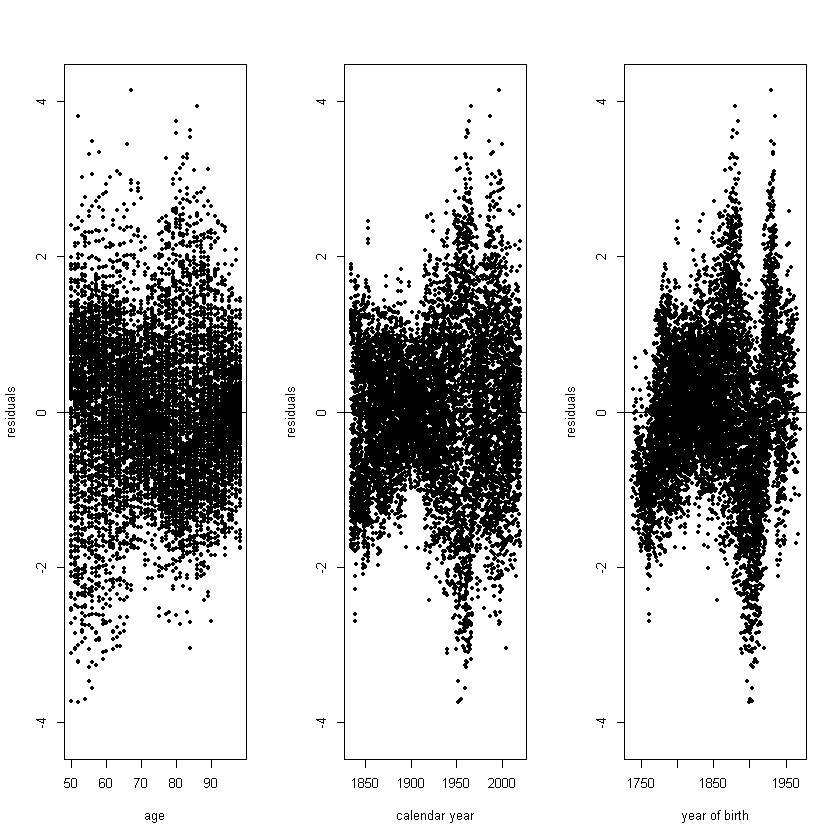
\includegraphics[scale =0.55]{output_11_0.png}
\end{figure}

lorsque l’on effectue un ajustement par la méthode de Lee-Carter, on peut analyser la variance des résidus, et confronter les observations à l’hypothèse d’homoscédasticité.

\section{Estimation des paramètres du modèle de CBD à partir des données historiques téléchargées} 
\begin{figure}[!htb]
 \caption{Danemark, modèle principal de CBD, homme de 50 à 98 ans}
    \centering
    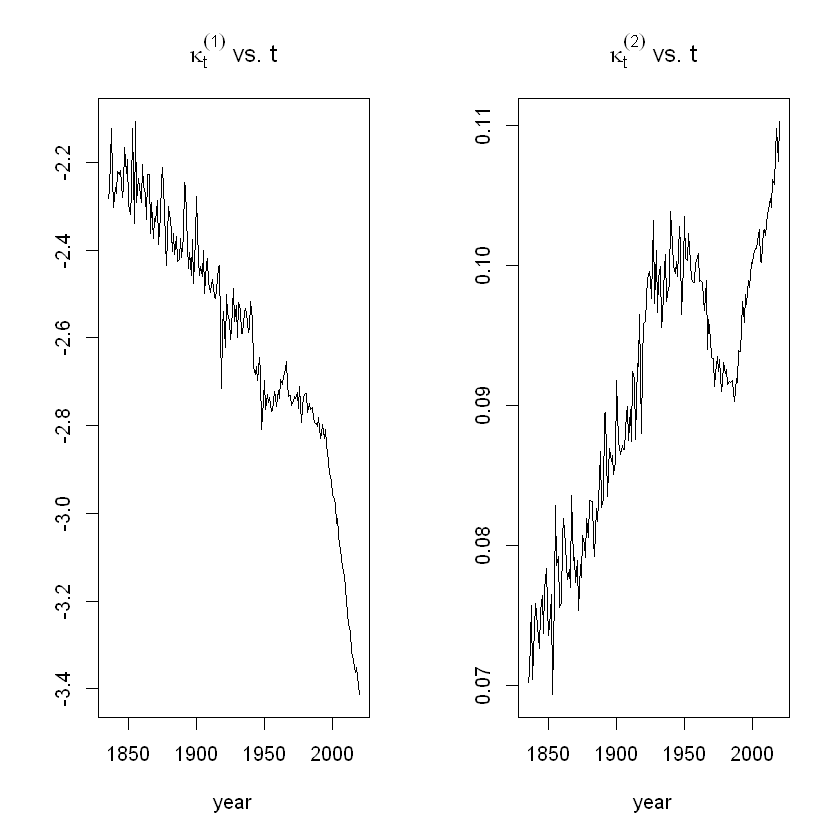
\includegraphics[scale =0.5]{output_18_7.png}
\end{figure}

\begin{figure}[!htb]
 \caption{Danemark, modèle principal de CBD, femme de 50 à 98 ans}
    \centering
    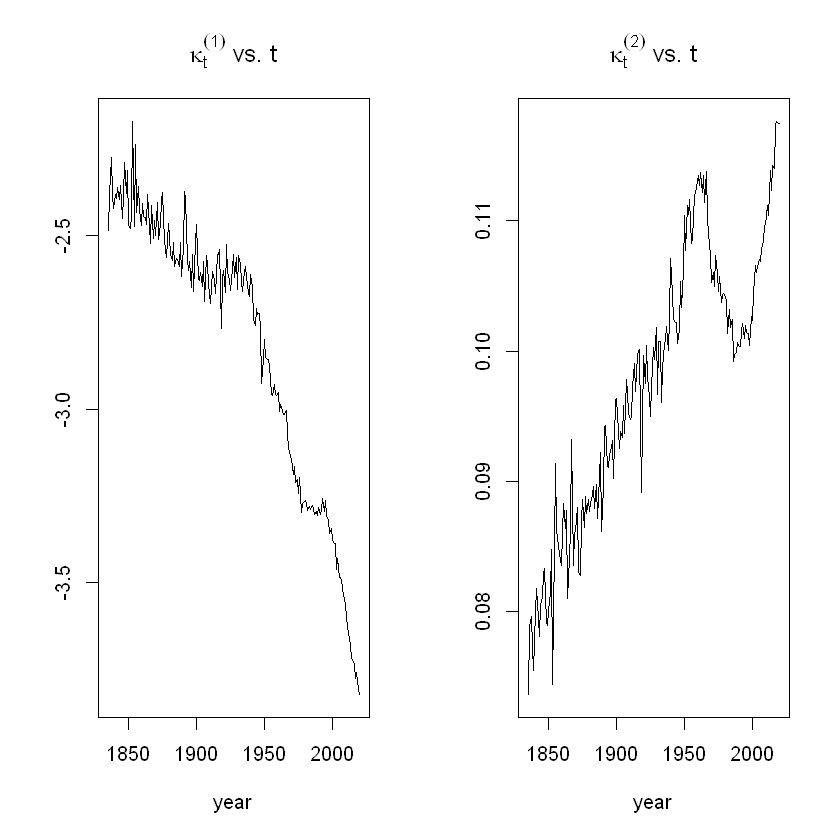
\includegraphics[scale =0.6]{output_18_9.png}
\end{figure}

\section{Log taux de mortalité estimés par le modèle Lee-Carter} 
\begin{figure}[!htb]
 \caption{log taux de mortalité (Danemark, 2010)}
    \centering
    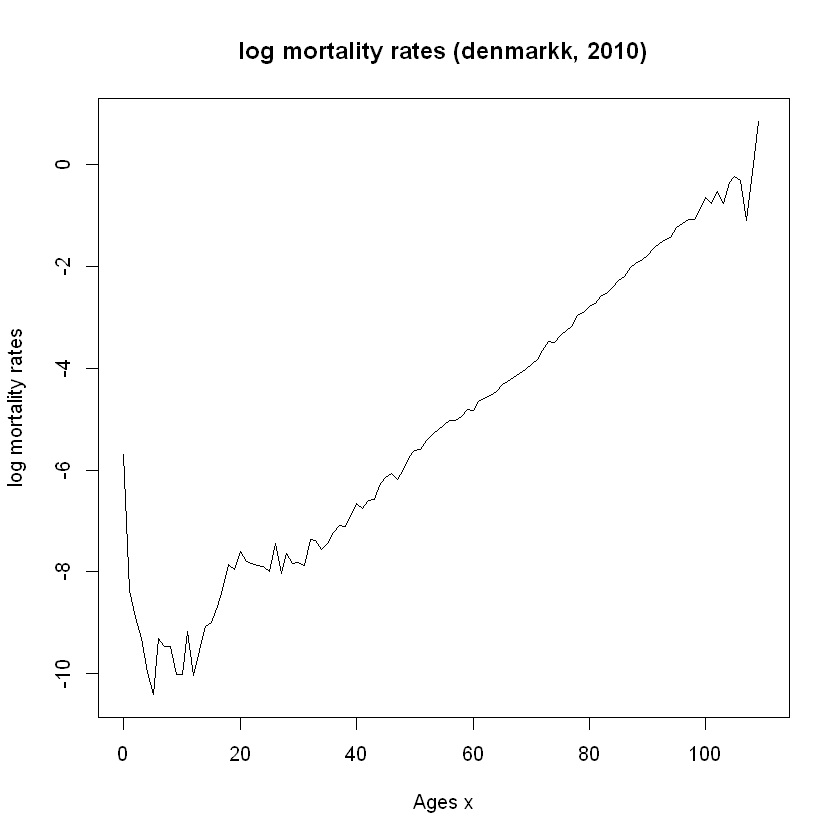
\includegraphics[scale =0.6]{output_20_0.png}
\end{figure}

\section{Procédure par défaut de projection des taux mortalité implémentée dans StMoMo}
Dans la famille des modèles de mortalité stochastique généralisés par âge, période et cohorte, la dynamique de la mortalité est les indices de période kt (i), i = 1, ..., N et l’indice de cohorte yt x. Par conséquent, les prévisions et la simulation des taux de mortalité nécessite la modélisation de ces indices à l’aide de séries chronologiques techniques. Pour les indices de période, nous envisageons deux approches de modélisation alternatives. Une première possibilité est d’utiliser l’approche standard dans la documentation actuarielle et de supposer que les indices de période suivent une multivariée marche aléatoire avec dérive.

\section{Projection des taux de mortalité à l’aide de la fonction forecast}
\begin{figure}[!htb]
 \caption{projection de taux de mortalité Danemark, homme sur 25 ans avec LCA}
    \centering
    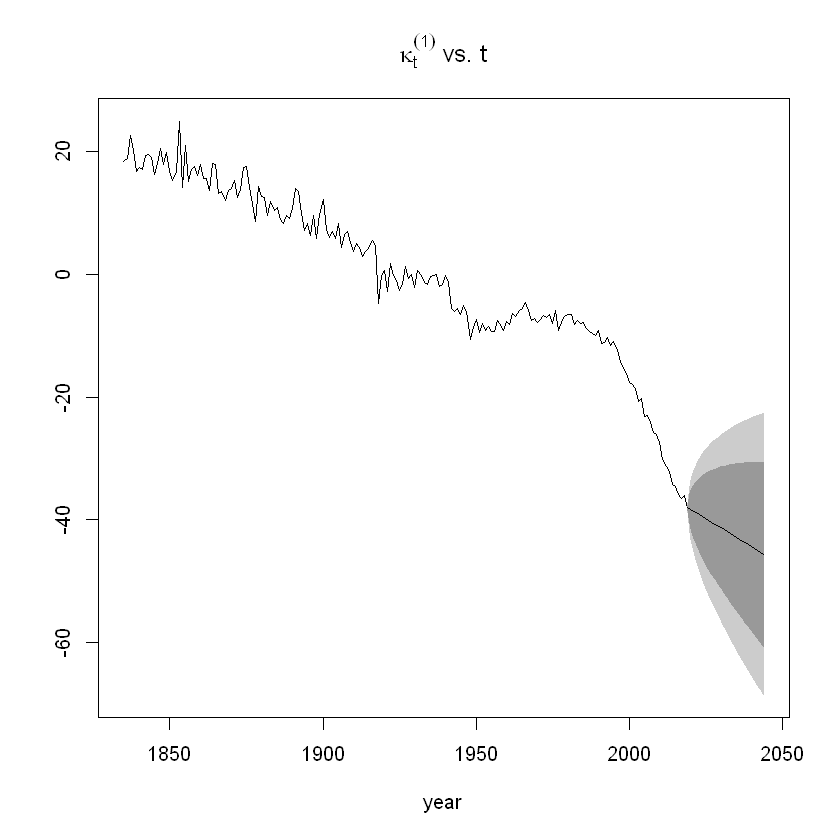
\includegraphics[scale =0.8]{output_24_1.png}
\end{figure}

\begin{figure}[!htb]
 \caption{projection de taux de mortalité Danemark, femme sur 25 ans avec LCA}
    \centering
    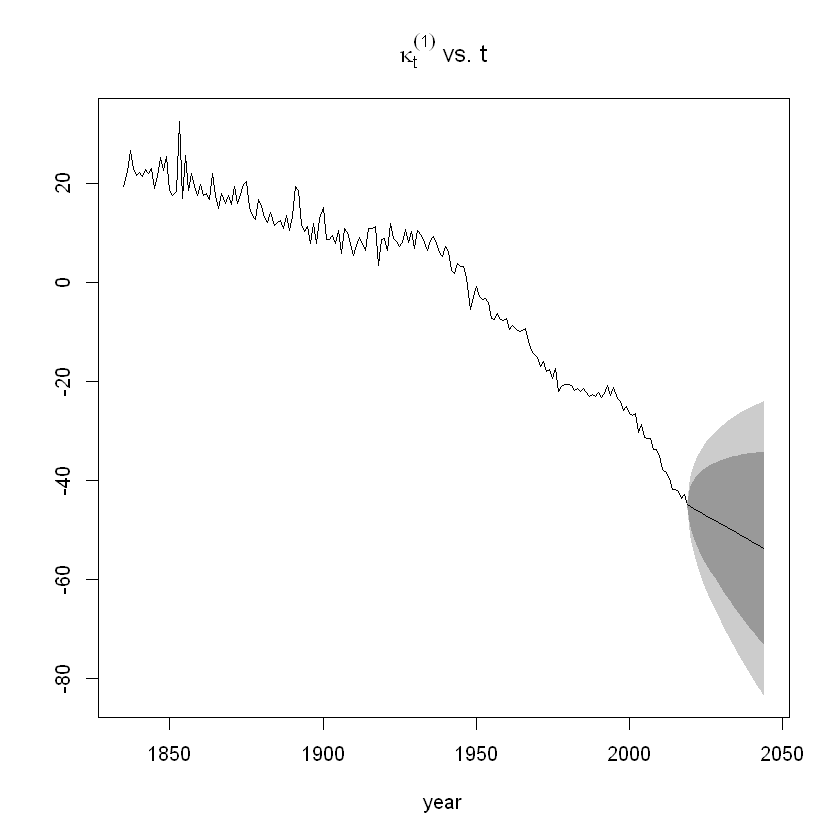
\includegraphics[scale =0.65]{output_24_2.png}
\end{figure}

\begin{figure}[!htb]
 \caption{projection de taux de mortalité Danemark, homme sur 25 ans avec CBD}
    \centering
    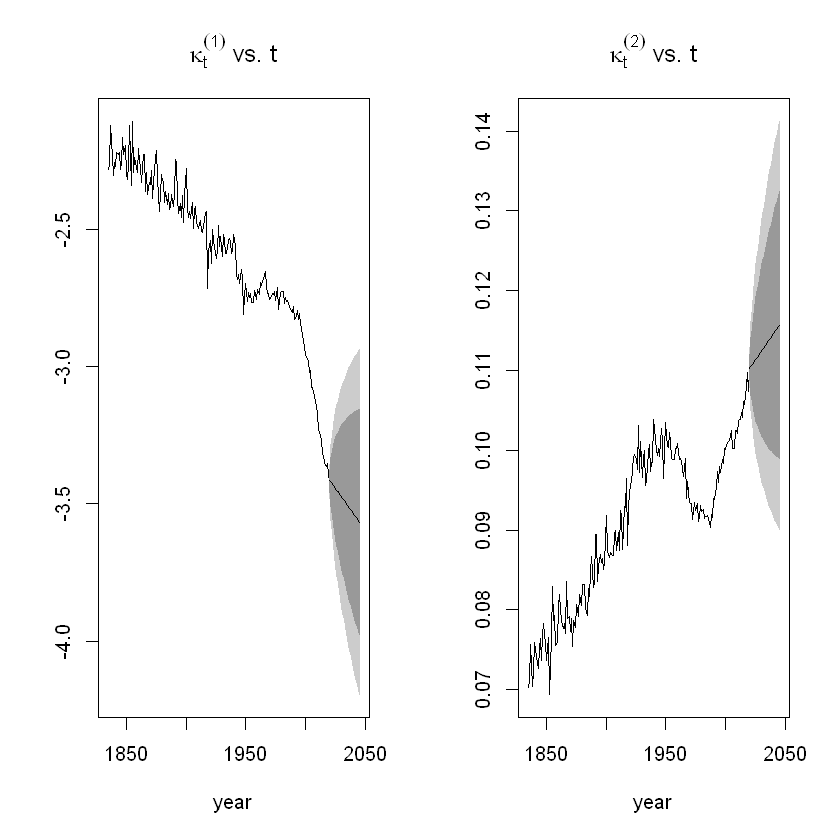
\includegraphics[scale =0.65]{output_25_0.png}
\end{figure}

\begin{figure}[!htb]
 \caption{projection de taux de mortalité Danemark, femme sur 25 ans avec CBD}
    \centering
    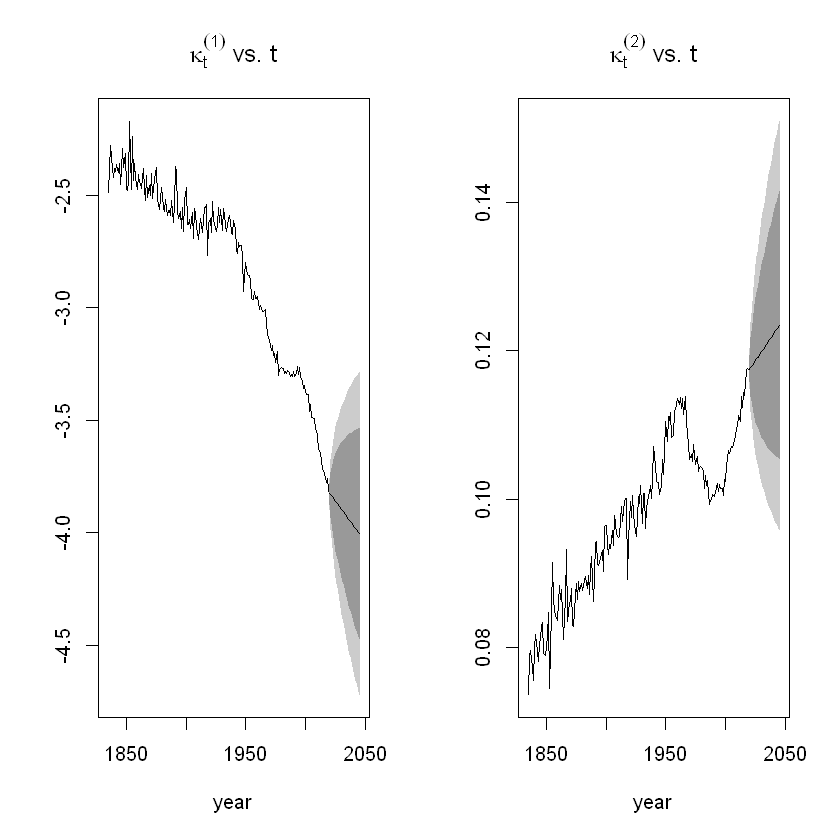
\includegraphics[scale =0.8]{output_25_1.png}
\end{figure}
        \clearpage
        
        \chapter*{Conclusion générale}
L’objectif de ce sujet était d’estimer et de projeter le taux de mortalité avec  les methodes Lee-Carter et CBD. Notre étude a été effectuer sur une population venant exactement de « Danemark » qui est une population assez spéciale dans le monde par ce qu’elle est caractérisée par plusieurs guerres d’où la baisse de taux de mortalité. Durant la période du projet on a essayé de traiter le sujet en répondant à des questions bien spécifique permettant de résoudre des problèmes d’actualités, on a estimé les taux de mortalité des hommes et des femmes en utilisant le modèle de Lee-carter et CBD qui sont Des références dans le domaine de prévision de mortalité qu’on a déjà estimé ses paramètres; à la fin notre groupe a essayé de comparer les deux modèles. 
Durant l'exploitation du taux de mortalité de la population danoise pour la période allant de 1876 jusqu'à 2019 nous avons constaté quelques instabilités pour des durées ou le pays a vécu des guerres, soit civile ou externe, cela avait un impact sur la variation du taux de mortalité de la Danemark.
Pour notre étude de cas et puisqu'on s'interesse à la population agés de plus que 50 ans nous avons opté à l'utilisation du modèle Cairn Blake Dowd qui est plus performant pour les cohortes possédant un age plutôt avancé. Selon la documentation fournie par la vigniette de StMoMo, il est conçu d'utiliser le modèle CBD pour la projection des taux de mortalité s'il s'agit d'une population agé et la durée de projection n'est pas assez large.
Dans notre cas nous avons constaté que le modèle CBD a présenté un intervale de confiance moin large que celui du modèle de Lee-Carter, maiscet intervalle couvre une période plus vaste au niveau du CBD que celui du Lee-Carter.
Pour conclure le projet a été très bénéfique pour tous les membres de l’équipe et nous a permis de découvrir de plus proche le monde d’actuariat vie en travaillant sur des données réelles.
        \clearpage
       
        
         %@author: Adam
	
\begin{thebibliography}{100}
\bibitem{BF} BusinessFrance; lien: https://www.businessfrance.fr/danemark-l-esperance-de-vie-continue-a-augmenter.

\bibitem{RA} Ressources Acturaielles. lien: http://www.ressources-actuarielles.net/EXT/ISFA/1226-02.nsf/9c8e3fd4d887\\4d60c1257052003eced6/ff3077c1f701b9b0c1257705004878f7/$\$$FILE/Namtchueng.pdf.

\bibitem{AM} A. Matoussi. (Année 2017-2018). Actuariat - Assurance vie chapitre 2 - Mortalité stochastique,
Université Le Mans (Maine) -’Institut du Risque et de l’Assurance du Mans.

\bibitem{SKAM} S.Kaakai - A. Matoussi (Année 2020-2021). Actuariat vie chapitre 3 - Mortalité stochastique,
ESPRIT (École Supérieure Privée d'Ingénierie et de Technologie).
\end{thebibliography} 

    
    
\end{document}